% Figure 1 - framework diagram, sized for a paper.
%
% Canvas 7.0in x 4.10in: drops in at \textwidth with NO scaling, so every
% size below is the size it prints at. No fontawesome dependency - the
% marks are drawn in TikZ, so they stay sharp and need no extra package.
%
%   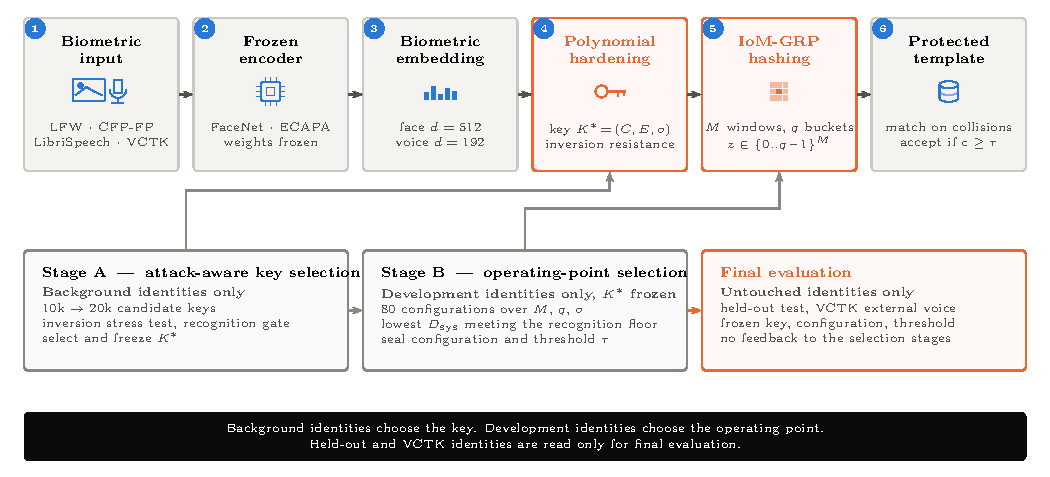
\includegraphics[width=\textwidth]{figure1_framework.pdf}
%
% No title inside the figure; the caption carries it, per paper
% convention.

\documentclass[10pt]{article}
\usepackage[paperwidth=7.0in,paperheight=3.18in,margin=0in]{geometry}
\usepackage{tikz}
\usepackage{xcolor}
\usepackage{amsmath}


\pagestyle{empty}
\setlength{\parindent}{0pt}
\setlength{\parskip}{0pt}
\setlength{\topskip}{0pt}
\usetikzlibrary{positioning,arrows.meta,calc}

% ---------- Palette: two accents plus neutrals ----------
\definecolor{Accent}{HTML}{2A78D6}
\definecolor{Keyed}{HTML}{EB6834}
\definecolor{Ink}{HTML}{0B0B0B}
\definecolor{Ink2}{HTML}{52514E}
\definecolor{Muted}{HTML}{898781}
\definecolor{Rule}{HTML}{C9C8C2}
\definecolor{Wash}{HTML}{F4F3EF}

\tikzset{
  stage/.style={
    rounded corners=2pt, minimum width=1.03in, minimum height=1.02in,
    inner sep=0pt, draw=Rule, line width=0.5pt, fill=Wash
  },
  keystage/.style={
    stage, draw=Keyed, line width=0.9pt, fill=Keyed!5
  },
  ttl/.style={
    font=\bfseries\fontsize{7}{8.2}\selectfont, text=Ink, align=center,
    anchor=north
  },
  body/.style={
    font=\fontsize{5.9}{7.1}\selectfont, text=Ink2, align=center,
    anchor=north
  },
  badge/.style={
    circle, inner sep=0pt, minimum size=0.135in, fill=#1,
    text=white, font=\bfseries\fontsize{5.2}{5.2}\selectfont
  },
  flow/.style={
    -{Stealth[length=1.6mm,width=1.15mm]}, draw=Ink2, line width=0.75pt
  },
  block/.style={
    rounded corners=2pt, minimum width=2.16in, minimum height=0.80in,
    draw=#1, fill=#1!4, line width=0.8pt, inner sep=0pt
  }
}

% ---------- Small vector marks (x, y, colour) ----------
\newcommand{\mkImage}[3]{\begin{scope}[shift={(#1,#2)}]
  \draw[#3,line width=0.5pt,rounded corners=0.4pt]
    (-0.105,-0.075) rectangle (0.105,0.075);
  \fill[#3] (-0.055,0.030) circle (0.018);
  \draw[#3,line width=0.5pt] (-0.09,-0.035) -- (-0.015,0.020)
    -- (0.035,-0.010) -- (0.09,-0.035);\end{scope}}

\newcommand{\mkMic}[3]{\begin{scope}[shift={(#1,#2)}]
  \draw[#3,line width=0.5pt,rounded corners=0.030]
    (-0.026,-0.010) rectangle (0.026,0.078);
  \draw[#3,line width=0.5pt] (-0.055,0.012) arc (180:360:0.055);
  \draw[#3,line width=0.5pt] (0,-0.043) -- (0,-0.075);
  \draw[#3,line width=0.5pt] (-0.040,-0.075) -- (0.040,-0.075);\end{scope}}

\newcommand{\mkChip}[3]{\begin{scope}[shift={(#1,#2)}]
  \draw[#3,line width=0.5pt,rounded corners=0.5pt]
    (-0.062,-0.062) rectangle (0.062,0.062);
  \draw[#3,line width=0.45pt,rounded corners=0.3pt]
    (-0.028,-0.028) rectangle (0.028,0.028);
  \foreach \k in {-0.035,0,0.035}{
    \draw[#3,line width=0.45pt] (\k,0.062) -- (\k,0.092);
    \draw[#3,line width=0.45pt] (\k,-0.062) -- (\k,-0.092);
    \draw[#3,line width=0.45pt] (0.062,\k) -- (0.092,\k);
    \draw[#3,line width=0.45pt] (-0.062,\k) -- (-0.092,\k);}\end{scope}}

\newcommand{\mkBars}[3]{\begin{scope}[shift={(#1,#2)}]
  \foreach \k/\h in {0/0.050,1/0.085,2/0.038,3/0.072,4/0.055}{
    \fill[#3] (-0.105+0.046*\k,-0.055) rectangle
      ++(0.028,\h);}\end{scope}}

\newcommand{\mkKey}[3]{\begin{scope}[shift={(#1,#2)}]
  \draw[#3,line width=0.6pt] (-0.055,0) circle (0.040);
  \draw[#3,line width=0.6pt] (-0.017,0) -- (0.105,0);
  \draw[#3,line width=0.6pt] (0.055,0) -- (0.055,-0.035);
  \draw[#3,line width=0.6pt] (0.095,0) -- (0.095,-0.028);\end{scope}}

\newcommand{\mkGrid}[3]{\begin{scope}[shift={(#1,#2)}]
  \foreach \r in {-1,0,1}{\foreach \c in {-1,0,1}{
    \fill[#3,opacity={ifthenelse(\r==0 && \c==0,1,0.45)}]
      (0.042*\c-0.016,0.042*\r-0.016) rectangle ++(0.032,0.032);}}
  \end{scope}}

\newcommand{\mkDB}[3]{\begin{scope}[shift={(#1,#2)}]
  \draw[#3,line width=0.55pt] (-0.062,0.045) arc (180:360:0.062 and 0.024);
  \draw[#3,line width=0.55pt] (-0.062,0.045) arc (180:0:0.062 and 0.024);
  \draw[#3,line width=0.55pt] (-0.062,0.045) -- (-0.062,-0.045);
  \draw[#3,line width=0.55pt] (0.062,0.045) -- (0.062,-0.045);
  \draw[#3,line width=0.55pt] (-0.062,-0.045) arc (180:360:0.062 and 0.024);
  \draw[#3,line width=0.5pt,opacity=0.55]
    (-0.062,0) arc (180:360:0.062 and 0.024);\end{scope}}

\begin{document}
\noindent
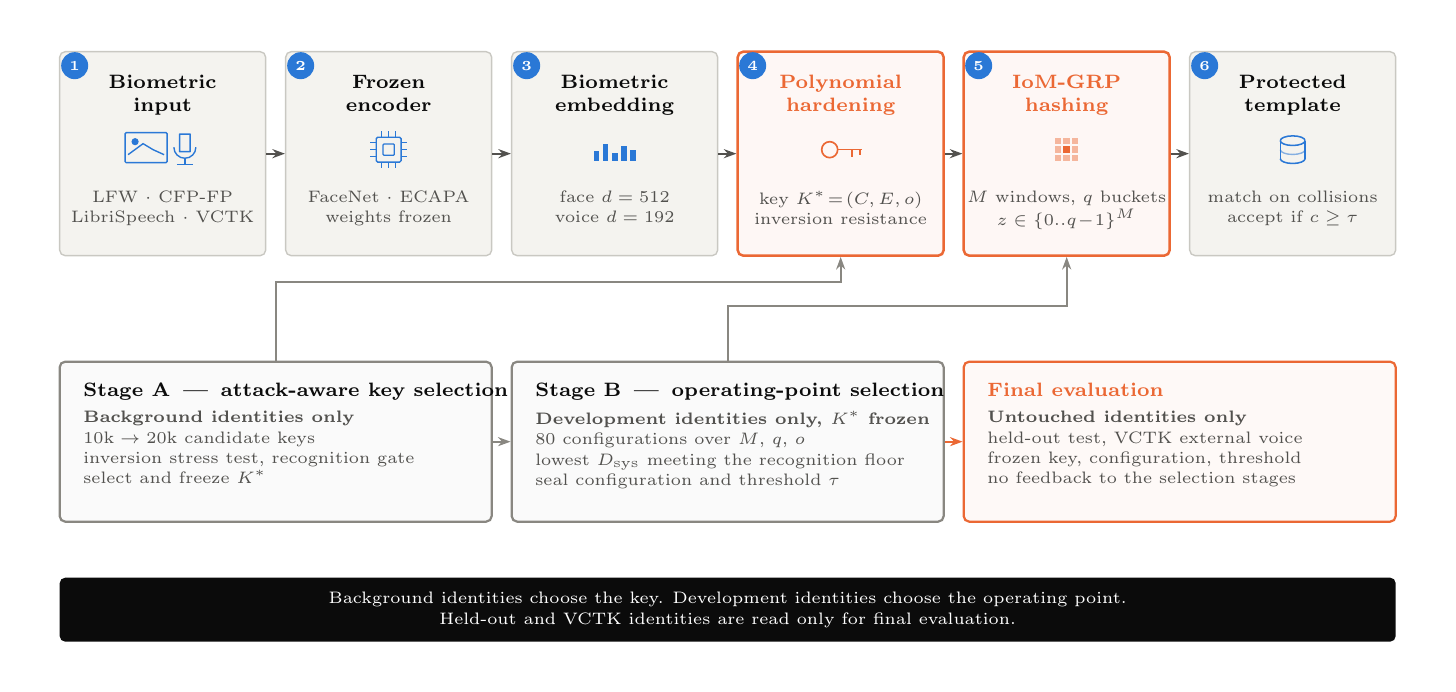
\begin{tikzpicture}[x=1in,y=1in]
\useasboundingbox (0,0.71) rectangle (7.0,3.89);

\def\cy{3.26}

% ---------- Pipeline ----------
\foreach \i/\x in {0/0.675,1/1.805,2/2.935,3/4.065,4/5.195,5/6.325}{
  \coordinate (S\i) at (\x,\cy);}

\node[stage]    (P0) at (S0) {};
\node[stage]    (P1) at (S1) {};
\node[stage]    (P2) at (S2) {};
\node[keystage] (P3) at (S3) {};
\node[keystage] (P4) at (S4) {};
\node[stage]    (P5) at (S5) {};

\node[ttl] at ([yshift=0.44in]S0) {Biometric\\input};
\node[ttl] at ([yshift=0.44in]S1) {Frozen\\encoder};
\node[ttl] at ([yshift=0.44in]S2) {Biometric\\embedding};
\node[ttl,text=Keyed] at ([yshift=0.44in]S3) {Polynomial\\hardening};
\node[ttl,text=Keyed] at ([yshift=0.44in]S4) {IoM-GRP\\hashing};
\node[ttl] at ([yshift=0.44in]S5) {Protected\\template};

\mkImage{0.592}{3.29}{Accent}
\mkMic{0.786}{3.28}{Accent}
\mkChip{1.805}{3.28}{Accent}
\mkBars{2.935}{3.28}{Accent}
\mkKey{4.065}{3.28}{Keyed}
\mkGrid{5.195}{3.28}{Keyed}
\mkDB{6.325}{3.28}{Accent}

\node[body] at ([yshift=-0.14in]S0) {LFW $\cdot$ CFP-FP\\LibriSpeech $\cdot$ VCTK};
\node[body] at ([yshift=-0.14in]S1) {FaceNet $\cdot$ ECAPA\\weights frozen};
\node[body] at ([yshift=-0.14in]S2) {face $d=512$\\voice $d=192$};
\node[body] at ([yshift=-0.14in]S3) {key $K^{\ast}\!=\!(C,E,o)$\\inversion resistance};
\node[body] at ([yshift=-0.14in]S4) {$M$ windows, $q$ buckets\\$z\in\{0..q\!-\!1\}^{M}$};
\node[body] at ([yshift=-0.14in]S5) {match on collisions\\accept if $c\geq\tau$};

\foreach \i in {0,...,5}{
  \pgfmathsetmacro{\bc}{\i<3 || \i>4 ? 0 : 1}
  \node[badge=Accent] at ([shift={(-0.44in,0.44in)}]S\i) {\number\numexpr\i+1\relax};}

\foreach \a/\b in {P0/P1,P1/P2,P2/P3,P3/P4,P4/P5}{
  \draw[flow] (\a.east) -- (\b.west);}

% ---------- Control blocks ----------
\node[block=Muted] (A) at (1.240,1.82) {};
\node[block=Muted] (B) at (3.500,1.82) {};
\node[block=Keyed] (C) at (5.760,1.82) {};

\foreach \n/\t/\c in {A/{Stage A\, \textemdash\, attack-aware key selection}/Ink,
                      B/{Stage B\, \textemdash\, operating-point selection}/Ink,
                      C/{Final evaluation}/Keyed}{
  \node[font=\bfseries\fontsize{6.6}{7.6}\selectfont,text=\c,
        anchor=north west] at ([shift={(0.075in,-0.065in)}]\n.north west) {\t};}

\node[font=\fontsize{5.9}{7.3}\selectfont,text=Ink2,anchor=north west,
      align=left] at ([shift={(0.075in,-0.205in)}]A.north west)
  {\textbf{Background identities only}\\
   $10\mathrm{k}\rightarrow20\mathrm{k}$ candidate keys\\
   inversion stress test, recognition gate\\
   select and freeze $K^{\ast}$};

\node[font=\fontsize{5.9}{7.3}\selectfont,text=Ink2,anchor=north west,
      align=left] at ([shift={(0.075in,-0.205in)}]B.north west)
  {\textbf{Development identities only, $K^{\ast}$ frozen}\\
   80 configurations over $M$, $q$, $o$\\
   lowest $D_{\mathrm{sys}}$ meeting the recognition floor\\
   seal configuration and threshold $\tau$};

\node[font=\fontsize{5.9}{7.3}\selectfont,text=Ink2,anchor=north west,
      align=left] at ([shift={(0.075in,-0.205in)}]C.north west)
  {\textbf{Untouched identities only}\\
   held-out test, VCTK external voice\\
   frozen key, configuration, threshold\\
   no feedback to the selection stages};

\draw[flow,draw=Muted] (A.east) -- (B.west);
\draw[flow,draw=Keyed] (B.east) -- (C.west);
\draw[flow,draw=Muted] (A.north) -- (1.240,2.62) -- (4.065,2.62) -- (P3.south);
\draw[flow,draw=Muted] (B.north) -- (3.500,2.50) -- (5.195,2.50) -- (P4.south);

% ---------- Principle strip ----------
\node[rounded corners=2pt,fill=Ink,text=white,minimum width=6.68in,
      minimum height=0.32in,font=\fontsize{6.2}{7.6}\selectfont,
      align=center] at (3.500,0.98)
  {Background identities choose the key. Development identities choose the
   operating point.\\Held-out and VCTK identities are read only for final
   evaluation.};

\end{tikzpicture}
\end{document}
